%% Main-Version Draft
\documentclass[11pt,epsf]{article}
%% -------------------------------
%% |          Packages           |
%% -------------------------------
 \usepackage{amsmath}
 \usepackage{graphicx}
 \usepackage[merge,numbers,compress]{natbib}
 \usepackage[T1]{fontenc}
 \usepackage{booktabs}
 \usepackage{xcolor} 
 \usepackage{xspace}
 \usepackage{dcolumn}
 \usepackage{hyperref}
 \usepackage{caption}
 \usepackage
 [subrefformat=parens,position=top,skip=-15pt,margin=15pt,justification=justified,singlelinecheck=false]
 {subcaption}

\setlength{\evensidemargin}{0cm}
\setlength{\oddsidemargin}{0cm}
\setlength{\topmargin}{0.00cm}
\setlength{\textwidth}{16.0cm}
\setlength{\textheight}{22.55cm}
\setlength{\headheight}{0cm}
\setlength{\headsep}{0cm}
\setlength{\voffset}{0cm}
\setlength{\paperheight}{27cm}

\renewcommand{\topfraction}{0.8}
\renewcommand{\bottomfraction}{0.5}
\renewcommand{\textfraction}{0.2}
\renewcommand{\floatpagefraction}{0.7}

\newcommand{\MP}[1]{{ {\color{blue}{ [MP: #1]}} }}

%% ---------------------------------
%% | ToDo Marker - only for draft! |
%% ---------------------------------
% Remove this section for final version!
\setlength{\marginparwidth}{20mm}

\newcommand{\margtodo}
{\marginpar{\textbf{\textcolor{red}{ToDo}}}{}}

\newcommand{\todo}[1]
{{\textbf{\textcolor{red}{(\margtodo{}#1)}}}{}}

\newcommand{\Pl}{\ell}
\newcommand{\fb}{{\ensuremath\unskip\,\text{fb}}\xspace}
% % new commands for cross referencing
\def\refeq#1{\mbox{(\ref{#1})}}
\def\reffi#1{\mbox{Figure~\ref{#1}}}
\def\reffis#1{\mbox{Figures~\ref{#1}}}
\def\refta#1{\mbox{Table~\ref{#1}}}
\def\reftas#1{\mbox{Tables~\ref{#1}}}
\def\refse#1{\mbox{Section~\ref{#1}}}
\def\refapp#1{\mbox{App.~\ref{#1}}}
\def\citere#1{\mbox{Ref.~\cite{#1}}}
\def\citeres#1{\mbox{Refs.~\cite{#1}}}

\newcommand{\ri}{\mathrm i}

\newcommand{\ie}{\emph{i.e.}\ }
\newcommand{\eg}{\emph{e.g.}\ }

\def\be{\begin{equation}}
\def\ee{\end{equation}}

\newcommand{\qqb}{\ensuremath{q\bar{q}}\xspace}
\newcommand{\PH}{\ensuremath{\text{H}}\xspace}
\newcommand{\Pj}{\ensuremath{\text{j}}\xspace}
\newcommand{\Pp}{\ensuremath{\text{p}}\xspace}
\newcommand{\Pe}{\ensuremath{\text{e}}\xspace}
\newcommand{\Pb}{\ensuremath{\text{b}}\xspace}
\newcommand{\Pq}{\ensuremath{\text{q}}\xspace}
\newcommand{\Pt}{\ensuremath{\text{t}}\xspace}
\newcommand{\Pu}{\ensuremath{\text{u}}\xspace}
\newcommand{\Pd}{\ensuremath{\text{d}}\xspace}
\newcommand{\Ps}{\ensuremath{\text{s}}\xspace}
\newcommand{\Pc}{\ensuremath{\text{c}}\xspace}
\newcommand{\Pg}{\ensuremath{\text{g}}\xspace}
\newcommand{\Pw}{\ensuremath{\text{w}}\xspace}
\newcommand{\PW}{\ensuremath{\text{W}}\xspace}
\newcommand{\PZ}{\ensuremath{\text{Z}}\xspace}
\newcommand{\Pbj}{\ensuremath{\text{j_b}}\xspace}
                                    
\newcommand{\Mt}{\ensuremath{m_\Pt}\xspace}
\newcommand{\MH}{\ensuremath{M_\PH}\xspace}
\newcommand{\MWOS}{\ensuremath{M_\PW^\text{OS}}\xspace}
\newcommand{\MW}{\ensuremath{M_\PW}\xspace}
\newcommand{\MZOS}{\ensuremath{M_\PZ^\text{OS}}\xspace}
\newcommand{\MZ}{\ensuremath{M_\PZ}\xspace}
\newcommand{\Mb}{\ensuremath{m_\Pb}\xspace}
\newcommand{\Gt}{\ensuremath{\Gamma_\Pt}\xspace}
\newcommand{\GH}{\ensuremath{\Gamma_\PH}\xspace}
\newcommand{\GZ}{\ensuremath{\Gamma_\PZ}\xspace}
\newcommand{\GZOS}{\ensuremath{\Gamma_\PZ^\text{OS}}\xspace}
\newcommand{\GW}{\ensuremath{\Gamma_\PW}\xspace}
\newcommand{\GWOS}{\ensuremath{\Gamma_\PW^\text{OS}}\xspace}

\newcommand{\MeV}{\ensuremath{\,\text{MeV}}\xspace}
\newcommand{\GeV}{\ensuremath{\,\text{GeV}}\xspace}
\newcommand{\TeV}{\ensuremath{\,\text{TeV}}\xspace}

\newcommand{\alphas}{\ensuremath{\alpha_\text{s}}\xspace}
\newcommand{\order}[1]{\ensuremath{\mathcal{O}{\left(#1\right)}}\xspace}

\newcommand{\abs}[1]{\left|#1\right|}
\newcommand{\deltar}{\ensuremath{\Delta R}\xspace}

\newcommand{\GF}{\ensuremath{G_\mu}}

\newcommand{\pt}{\ensuremath{p_\text{T}}\xspace}
\newcommand{\ptsub}[1]{\ensuremath{p_{\text{T},#1}}\xspace}

\renewcommand{\Re}{\mathop{\mathrm{Re}}\nolimits}
\renewcommand{\Im}{\mathop{\mathrm{Im}}\nolimits}

\newcommand{\MVOS}{\ensuremath{M_{V}^\text{OS}}\xspace}%
\newcommand{\GVOS}{\ensuremath{\Gamma_{V}^\text{OS}}\xspace}%

\newcommand{\sq}{\tilde{q}}
\newcommand{\su}{\tilde{u}}
\newcommand{\sd}{\tilde{d}}
\newcommand{\gl}{\tilde{g}}
\def\bom#1{{\mbox{\boldmath $#1$}}}
\newcommand\nn         {\nonumber}
\newcommand{\sul}{\tilde{u}_L}
\newcommand{\scl}{\tilde{c}_L}
\newcommand{\sdl}{\tilde{d}_L}
\newcommand{\ssl}{\tilde{s}_L}
\newcommand{\sur}{\tilde{u}_R}
%\newcommand{\scr}{\tilde{c}_R}
\newcommand{\sdr}{\tilde{d}_R}
\newcommand{\ssr}{\tilde{s}_R}
\newcommand{\stone}{\tilde{t}_1}
\newcommand{\sbone}{\tilde{b}_1}
\newcommand{\sttwo}{\tilde{t}_2}
\newcommand{\sbtwo}{\tilde{b}_2}
\newcommand{\neutone}{\tilde{\chi}^0_1}
\newcommand\sss{\mathchoice%
{\displaystyle}%
{\scriptstyle}%
{\scriptscriptstyle}%
{\scriptscriptstyle}%
}
\newcommand{\newc}{\newcommand}
% \newc{\be}{\begin{equation}}
% \newc{\ee}{\end{equation}}
\newc{\bi}{\begin{itemize}}
\newc{\ei}{\end{itemize}}
\newc{\benu}{\begin{enumerate}}
\newc{\eenu}{\end{enumerate}}
\newc{\bc}{\begin{center}}
\newc{\ec}{\end{center}}
\newc{\bfig}{\begin{figure}}
\newc{\efig}{\end{figure}}
\newc{\qbar}{\bar{q}}
\newc{\go}{\tilde{g}}
\newc{\PB}{\textsc{Powheg-Box}}
\newcommand\matB{{\cal B}}
\newcommand\matR{{\cal R}}
\newcommand\matV{{\cal V}}
\newcommand\matO{{\cal O}}
\newcommand\matF{{\cal F}}

\newcommand{\Recola}{{\sc Recola}\xspace}
\newcommand{\Sherpa}{{\sc Sherpa}\xspace}
\newcommand{\Rivet}{{\sc Rivet}\xspace}
\newcommand{\Amegic}{A\protect\scalebox{0.8}{MEGIC}\xspace}
\newcommand{\Comix}{C\protect\scalebox{0.8}{OMIX}\xspace}
\newcommand{\OpenLoops}{O\protect\scalebox{0.8}{PEN}L\protect\scalebox{0.8}{OOPS}\xspace}
\newcommand{\Njet}{N\protect\scalebox{0.8}{JET}\xspace}
\newcommand{\BlackHat}{B\protect\scalebox{0.8}{LACK}H\protect\scalebox{0.8}{AT}\xspace}
\newcommand{\Gosam}{G\protect\scalebox{0.8}{O}S\protect\scalebox{0.8}{AM}\xspace}
\newcommand{\mocanlo}{{\sc MoCaNLO}\xspace}
\newcommand{\collier}{{\sc Collier}\xspace}
\newcommand{\CutTools}{{\sc CutTools}\xspace}
\newcommand{\madgraph}{{\sc\small MadGraph5\_aMC@NLO}\xspace}
\newcommand{\madgraphbis}{{\sc\small MG5\_aMC@NLO}\xspace}
\newcommand{\rT}{{\mathrm{T}}}
\newcolumntype{.}{D{.}{.}{-1}}
\newcolumntype{d}[1]{D{.}{.}{#1}}

\renewcommand{\vec}[1]{\mathbf{#1}}
\colorlet{tableoverheadcolor}{gray!37.5}
\colorlet{tableheadcolor}{gray!25}
\colorlet{tablerowcolor}{gray!12.5}

\newcommand{\lsim}
{\;\raisebox{-.3em}{$\stackrel{\displaystyle <}{\sim}$}\;}
\newcommand{\gsim}
{\;\raisebox{-.3em}{$\stackrel{\displaystyle >}{\sim}$}\;}
\def\asymp#1{\;\raisebox{-.4em}{$\widetilde{\scriptstyle #1}$}\;}

\newlength{\width}
\newlength{\height}
\newcommand{\brabar}[1]{%
    \settoheight{\height}{\ensuremath{#1}}%
    \settowidth{\width}{\ensuremath{#1}}%
    \makebox[0pt][l]{\ensuremath{#1}}%
    \raisebox{1.26ex}{\scalebox{.3}{\textbf{(}}}%
    \rule[1.41\height]{0.7\width}{0.35pt}%
    \raisebox{1.26ex}{\scalebox{.3}{\textbf{)}}}%
}

% modifications for drafts for drafts
\newcommand{\mpar}[1]{{\marginpar{\hbadness10000%
                      \sloppy\hfuzz10pt\boldmath\bf\textcolor{red}{#1}}}%
                      \typeout{marginpar: #1}\ignorespaces}
\marginparwidth 1.2cm
\marginparsep 0.2cm
\def\draftdate{\relax}
\def\mda{\relax}
\def\mua{\relax}
\def\mla{\relax}
\def\draft{
\def\thtystars{******************************}
\def\sixtystars{\thtystars\thtystars}
\typeout{}
\typeout{\sixtystars**}
\typeout{* Draft mode!
         For final version remove \protect\draft\space in source file *}
\typeout{\sixtystars**}
\typeout{}
\def\draftdate{\today}
\def\mua{\marginpar[\boldmath\hfil$\uparrow$]%
                   {\boldmath$\uparrow$\hfil}\color{black}%
                    \typeout{marginpar: $\uparrow$}\ignorespaces}
\def\mda{\color{red}\marginpar[\boldmath\hfil$\downarrow$]%
                   {\boldmath$\downarrow$\hfil}%
                    \typeout{marginpar: $\downarrow$}\ignorespaces}
\def\mla{\marginpar[\boldmath\hfil$\rightarrow$]%
                   {\boldmath$\leftarrow $\hfil}%
                    \typeout{marginpar: $\leftrightarrow$}\ignorespaces}
\def\Mua{\marginpar[\boldmath\hfil$\Uparrow$]%
                   {\boldmath$\Uparrow$\hfil}\color{black}%
                    \typeout{marginpar: $\uparrow$}\ignorespaces}
\def\Mda{\color{red}\marginpar[\boldmath\hfil$\Downarrow$]%
                   {\boldmath$\Downarrow$\hfil}%
                    \typeout{marginpar: $\downarrow$}\ignorespaces}
\def\Mla{\marginpar[\boldmath\hfil\textcolor{red}{$\Rightarrow$}]%
                   {\boldmath\textcolor{red}{$\Leftarrow $}\hfil}%
                    \typeout{marginpar: $\leftrightarrow$}\ignorespaces}
\overfullrule 5pt
\oddsidemargin 15mm
\marginparwidth 29mm
}

% switch on draft mode
%\draft



\begin{document}

\title{\hfill ~\\[-30mm]
\phantom{h} \hfill\mbox{\small PREPRINT}
\\[1cm]
\vspace{13mm}   \textbf{VBS for HE and HL LHC}}

\date{}
\author{
Ansgar Denner$^{1\,}$\footnote{E-mail:
  \texttt{ansgar.denner@physik.uni-wuerzburg.de}},
Mathieu Pellen$^{1\,, 2\,}$\footnote{E-mail:
  \texttt{mathieu.pellen@physik.uni-wuerzburg.de}},
Michael Rauch
\\[9mm]
{\small\it
$^1$Universit\"at W\"urzburg, %
        Institut f\"ur Theoretische Physik und Astrophysik,} \\ %
{\small\it Emil-Hilb-Weg 22, \linebreak %
        97074 W\"urzburg, %
        Germany}\\[3mm]
{\small\it
$^2$University of Cambridge, Cavendish Laboratory,} \\ %
{\small\it Cambridge CB3 0HE, United Kingdom}\\[3mm]
}

\maketitle

\begin{abstract}
\noindent

\end{abstract}
\thispagestyle{empty}
\vfill
\newpage
\setcounter{page}{1}

\tableofcontents
\newpage


\section{Introduction}

The measurement of vector-boson scattering (VBS) processes is one of
the most important tasks in the future Large Hadron Collider (LHC) program.
The expected experimental precision allows precise measurements.
This offers great opportunities to probe the electroweak (EW) sector and its associated symmetry breaking mechanism
(see Refs.~\cite{Mangano:2016jyj,Goncalves:2017gzy,Jager:2017owh} for $100\TeV$-collider studies).
Therefore, it is of prime importance to make precise theoretical
predictions available for the future operation of the LHC.
In this contribution, predictions for NLO QCD and EW corrections are provided for the LHC running in its high-luminosity (HL) and high-energy (HE) configurations.
The HL set-up corresponds to a centre-of-mass energy of $14\TeV$ while
the HE one refers to $27\TeV$.
For both centre-of-mass energies the same type of event selections has been used.
These predictions represent important benchmarks as they indicate the expected rates and the corresponding theoretical uncertainties.
The QCD corrections are particularly important as they can significantly distort the shape of jet-related observables \cite{Jager:2006zc,Jager:2006cp,Bozzi:2007ur,Jager:2009xx,Jager:2011ms,Denner:2012dz,Rauch:2016pai,Biedermann:2017bss,Ballestrero:2018anz}.
In addition, the inclusion of NLO QCD corrections reduces the theoretical uncertainties.
The NLO EW corrections have been shown to be very large for VBS processes \cite{Biedermann:2016yds} and even the dominating NLO contribution for same-sign WW scattering \cite{Biedermann:2017bss}.

In this study, the NLO QCD corrections have been obtained based on Refs.~\cite{Arnold:2008rz, Arnold:2011wj, Baglio:2014uba} in the so-called VBS approximation \cite{Oleari:2003tc,Denner:2012dz,Ballestrero:2018anz}.
The NLO EW corrections have been obtained from {\sc MoCaNLO+Recola}
\cite{Bendavid:2018nar,Actis:2016mpe,Actis:2016mpe} based on a
full NLO computation \cite{Biedermann:2017bss}.
The differences between the full computation and the one based on the
VBS approximation have been found to be below the per-cent level at
NLO QCD \cite{Ballestrero:2018anz}.
This justifies the combination of the NLO corrections from these two types of calculations.
The QCD corrections have been computed for all possible VBS signatures, while the EW ones are only known for same-sign WW scattering.
While the exact value of the corrections is expected to be different
for other signatures, their magnitudes and nature should be similar.

\section{Set-up}

The hadronic scattering processes are simulated at the LHC with a centre-of-mass energies $\sqrt s = 14 \TeV$ and $\sqrt s = 27 \TeV$.
    The NNNPDF~3.1 LUXQED parton distribution
    functions~(PDFs)~\cite{Bertone:2017bme} with five massless
    flavours,\footnote{For the process considered, no bottom
      (anti-)quarks appear in the initial or final state at LO and
      NLO, as they would lead to top quarks rather than light jets in the final state.} 
    NLO-QCD evolution, and a strong coupling constant $\alphas\left( \MZ \right) = 0.118$ are employed.\footnote{The corresponding identifier {\tt lhaid} in the program LHAPDF6~\cite{Buckley:2014ana} is 324900.}
    Initial-state collinear singularities are factorised according to
    the ${\overline{\rm MS}}$ scheme, consistently with the conventions in the NNPDF set.

 The other input parameters have been chosen as in Ref.~\cite{Ballestrero:2018anz}.
    For the massive particles, the following masses and decay widths are used:
    %
    \begin{alignat}{2}
                      \Mt   &=  173.21\GeV,       & \quad \quad \quad \Gt &= 0 \GeV,  \nonumber \\
                    \MZOS &=  91.1876\GeV,      & \quad \quad \quad \GZOS &= 2.4952\GeV,  \nonumber \\
                    \MWOS &=  80.385\GeV,       & \GWOS &= 2.085\GeV,  \nonumber \\
                    M_{\rm H} &=  125.0\GeV,       &  \GH   &=  4.07 \times 10^{-3}\GeV.
    \end{alignat}
    %
    The measured on-shell (OS) values for the masses and widths of the W and Z bosons are converted into pole values for the gauge bosons ($V=\PW,\PZ$) according to Ref.~\cite{Bardin:1988xt},
    %
    \begin{equation}
    \begin{split}
            M_V &= \MVOS/\sqrt{1+(\GVOS/\MVOS)^2}\,, \\
       \Gamma_V &= \GVOS/\sqrt{1+(\GVOS/\MVOS)^2}.
    \end{split}
    \end{equation}
    %
    The EW coupling is fixed in the $G_\mu$ scheme \cite{Denner:2000bj} according to 
    \begin{equation}
    \alpha =  \frac{\sqrt{2}}{\pi} G_{\mu} M_{\rm W}^2 \left(1-\frac{M_{\rm W}^2}{M_{\rm Z}^2} \right),
    \end{equation}
    with
    %
    \begin{equation}
        G_{\mu}    = 1.16637\times 10^{-5}\GeV^{-2},
    \end{equation}
    %
    and $M_V^2$ corresponds to the real part of the squared pole mass.
    The numerical value of $\alpha$ corresponding to this choice of input parameters is
    %
    \begin{equation}
     1/\alpha = 132.3572\ldots\,.
    \end{equation}
    The Cabibbo--Kobayashi--Maskawa matrix is assumed to be diagonal, meaning that the mixing between different quark generations is neglected.
    The complex-mass scheme~\cite{Denner:1999gp,Denner:2005fg,Denner:2006ic} is used throughout to treat unstable intermediate particles in a gauge-invariant manner.

    The central value of the renormalisation and factorisation scales is set to 
    %
    \begin{equation}
    \label{eq:defscale}
     \mu_{\rm ren} = \mu_{\rm fac} = \sqrt{p_{\rm T, j_1}\, p_{\rm T, j_2}} .
    \end{equation}
    %
    The transverse momenta are those of the two hardest jets.
    This choice of scale has been shown to provide stable NLO-QCD predictions \cite{Denner:2012dz}.

    Following experimental measurements \cite{Aad:2014zda,Aaboud:2016ffv,Khachatryan:2014sta,CMS:2017adb} and prospect studies \cite{ATL-PHYS-PUB-2017-023}, the event selection used in the present study is:

    \begin{itemize}
        \item The two same-sign charged leptons are required to fulfil
          cuts on transverse momentum, rapidity, separation in the
          rapidity--azimuthal-angle, and the lepton-pair invariant mass, 
            \begin{align}
            \label{cut:1}
             \ptsub{\Pl} >  20\GeV,\qquad |y_{\Pl}| < 4.0, \qquad \Delta R_{\Pl\Pl}> 0.3, \qquad m_{\Pl\Pl}>20\GeV.
            \end{align}
            %
        \item The total missing transverse momentum, computed from the vectorial sum of the transverse momenta of the two neutrinos, is required to be
            \begin{align}
            \label{cut:2}
              p_{\rm T, miss} >  40\GeV\,.
            \end{align}
            %
        \item QCD partons (light quarks and gluons) are clustered  using the anti-$k_T$ algorithm~\cite{Cacciari:2008gp} with jet-resolution parameter $R=0.4$.
        We impose cuts on the jets' transverse momenta and rapidities,  
            \begin{align}
            \label{cut:3}
             \ptsub{\Pj} >  30\GeV, \qquad |y_\Pj| < 4.0. 
            \end{align}
            VBS cuts are applied on the two jets with largest transverse momentum, unless otherwise stated. In particular, we impose a cut on the 
             in\-vari\-ant mass of the di-jet system, as well as on the rapidity separation of the two jets and their separation from leptons,
            \begin{align}
            \label{cut:4}
             m_{\Pj \Pj} >  500\GeV,\qquad |\Delta y_{\Pj \Pj}| > 2.5, \qquad \Delta R_{\Pj\Pl} > 0.3 .
            \end{align}
            %
        \item Finally, the centrality of the leptons is enforced as defined in Ref.~\cite{ATL-PHYS-PUB-2017-023}:
            \begin{align}
            \label{cut:5}
             \zeta = \text{min}\left[\text{min}\left(y_{\Pl_1},y_{\Pl_2}\right) - \text{min}\left(y_{\Pj_1},y_{\Pj_2}\right), \text{max}\left(y_{\Pj_1},y_{\Pj_2}\right) - \text{max}\left(y_{\Pl_1},y_{\Pl_2}\right)\right]> 0 .
            \end{align}
            
        \item When EW corrections are computed, real photons and charged fermions are clustered using the anti-$k_T$ algorithm with
            radius parameter $R=0.1$. In this case, leptons and quarks are understood as {\it dressed fermions}.
    \end{itemize}

\section{Discussion}


In this section we focus on the discussion of Standard Model predictions for the HL and HE LHC.
This entails both QCD and EW corrections that have been combined together.

For VBS processes EW corrections are particularly large and therefore of prime importance.
The leading contributions originate from the exchange of massive gauge bosons in the virtual corrections.
They tend to grow large and negative in the high-energy limit owing to
so-called Sudakov double logarithms.
As shown in Ref.~\cite{Biedermann:2016yds}, large EW corrections are an intrinsic feature of VBS at the LHC.
While this study is based on the same-sign $\PW$ channel, it
has been further confirmed recently by the computation of large EW corrections to the $\PW\PZ$ channel \cite{SchwanTalk,dittmaieretla}.

Given their size and the foreseen experimental
precision, these corrections are actually measurable.
Because they involve interactions of the EW sector, their measurement would constitute a further test of the SM.
On the left hand-side of Fig.~\ref{fig:ew}, the distribution in the invariant mass of the two leading jets is shown at LO and NLO EW for the process $\Pp\Pp \to \mu^+ \nu_{\mu} \Pe^+ \nu_{\Pe} \Pj\Pj$ at $14\TeV$.
The yellow band describes the expected statistical uncertainty for a
HL LHC collecting $3000\fb^{-1}$ based on a relative variation of $\pm1/N_{\rm obs}$ where $N_{\rm obs}$ is the number of observed events in each bin.
On the right hand-side for Fig.~\ref{fig:ew}, a similar plot for the absolute rapidity of the jet pair is shown.
It is thus clear that with the expected luminosity, one is not only
sensitive to the VBS process but also to its EW corrections.
%
\begin{figure}
% \hspace{-2cm}
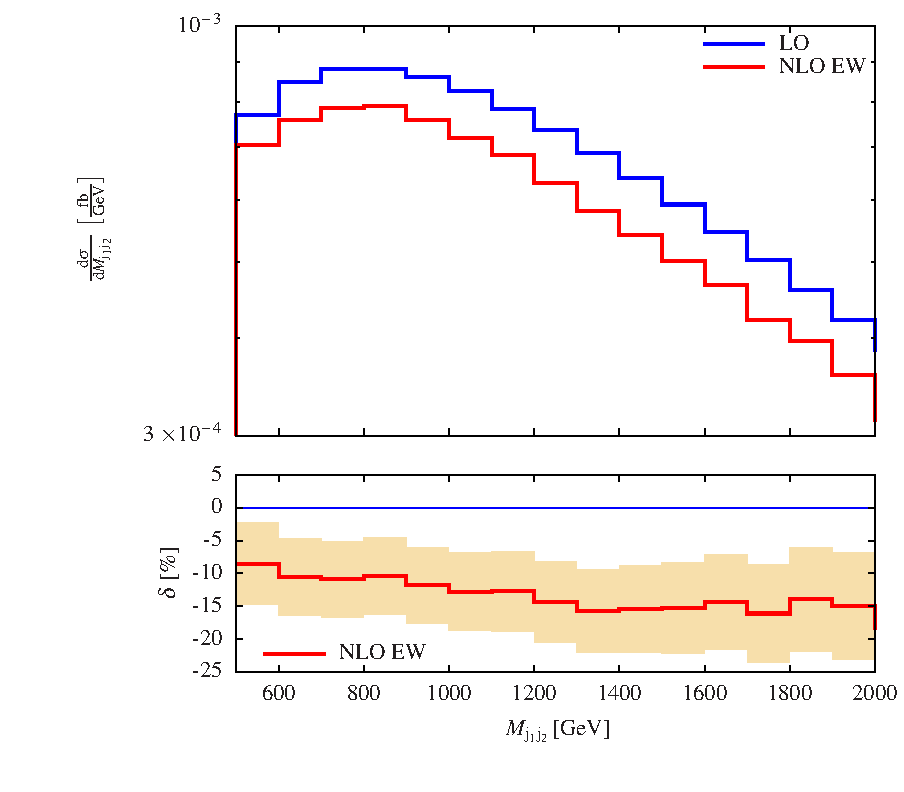
\includegraphics[width=.5\textwidth]{{{Figures/histogram_invariant_mass_mjj12_rauch}}}
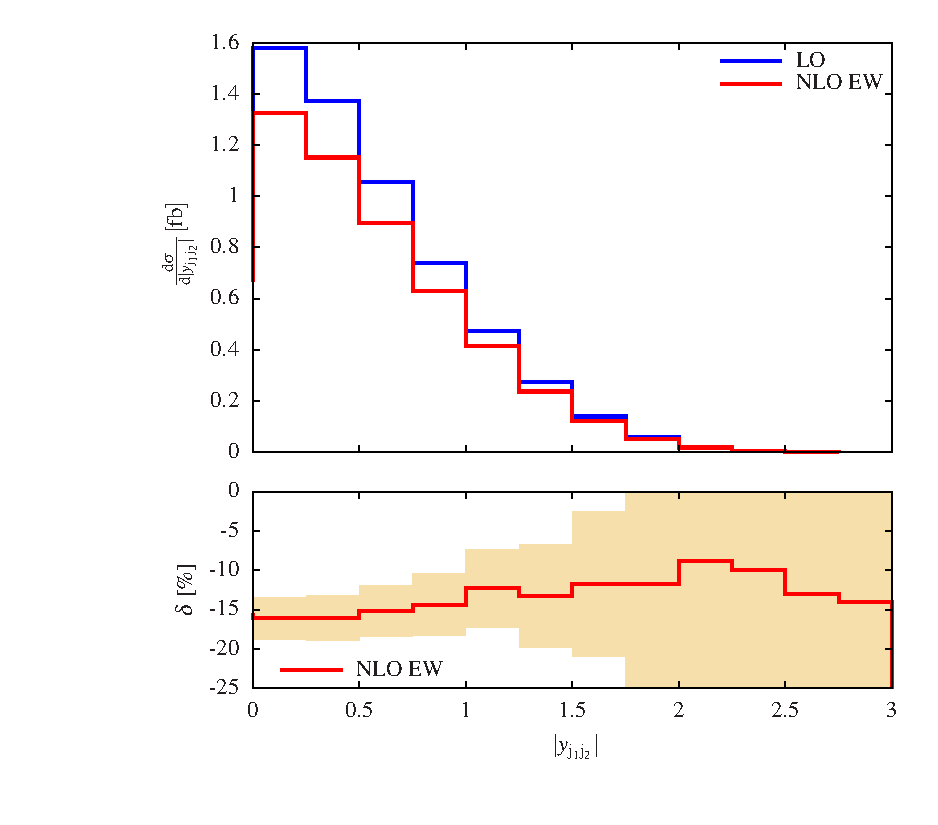
\includegraphics[width=.5\textwidth]{{{Figures/histogram_rapidity_j1j2}}}
% \vspace*{-1em}
\caption{
Differential distributions in the invariant mass of the two jets (left) and their rapidity (right)
in $\Pp\Pp\to\mu^+\nu_\mu\Pe^+\nu_{\Pe}\Pj\Pj$ at $14\TeV$ including NLO EW corrections (upper panel) and relative NLO EW corrections (lower panel).
The yellow band describes the expected statistical
uncertainty for a high-luminosity LHC collecting $3000\fb^{-1}$ and
represents a relative variation of $\pm 1/\sqrt{N_{\rm obs}}$ where $N_{\rm obs}$ is the number of observed events in each bin.
}
\label{fig:ew}
\end{figure}

\begin{figure}
% \hspace{-2cm}
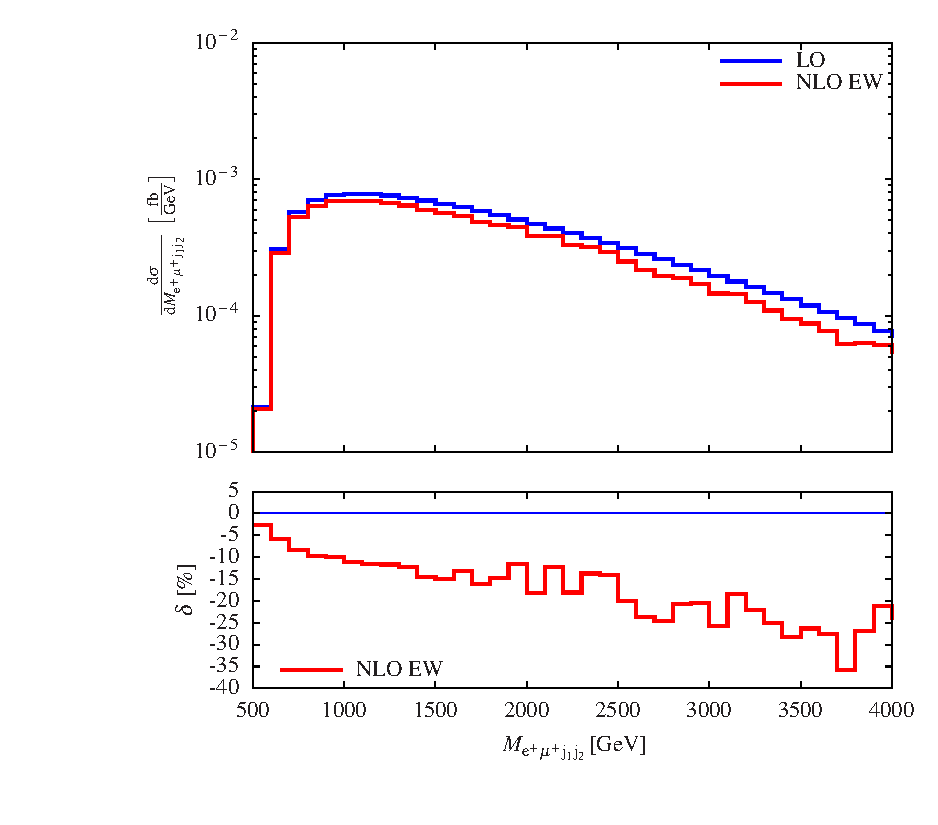
\includegraphics[width=.5\textwidth]{{{Figures/histogram_invariant_mass_all_HL}}}
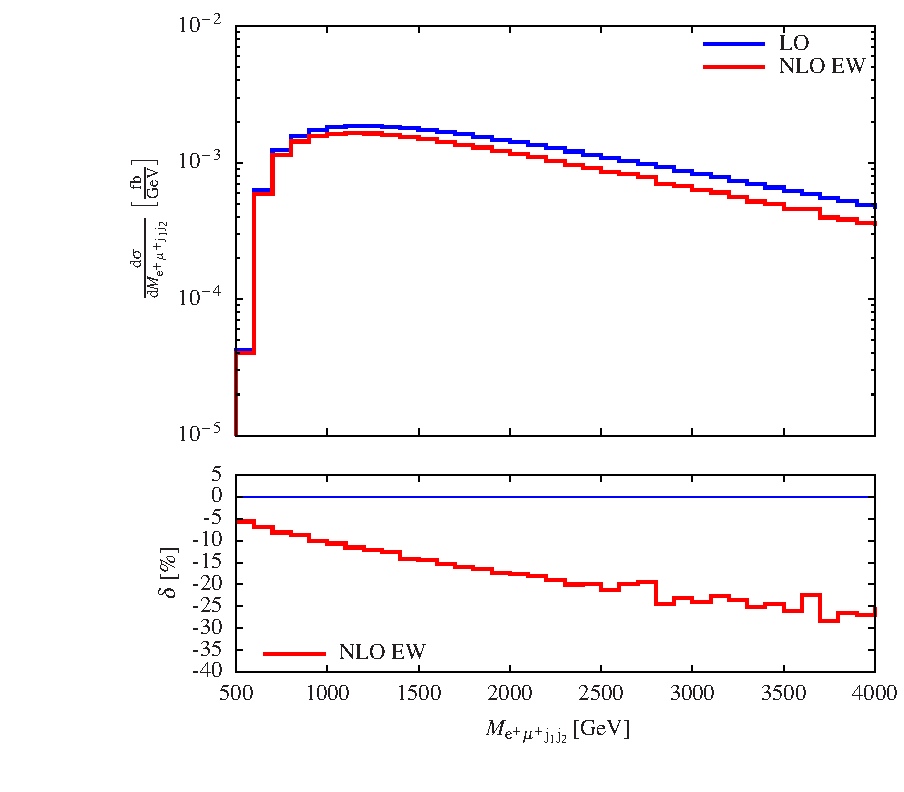
\includegraphics[width=.5\textwidth]{{{Figures/histogram_invariant_mass_all_HE}}}
% \vspace*{-1em}
\caption{
Differential distribution in the invariant mass of the visible system ($\Pe^+\mu^+\Pj\Pj$) in $\Pp\Pp\to\mu^+\nu_\mu\Pe^+\nu_{\Pe}\Pj\Pj$ at $14\TeV$ (left) and $27\TeV$ (right) including NLO EW corrections (upper panel) and relative NLO EW corrections (lower panel).
}
\label{fig:ew2}
\end{figure}

In Fig.~\ref{fig:ew2}, the distributions in the invariant mass of the visible system ($\Pe^+\mu^+\Pj\Pj$) at both $14\TeV$ (left) and $27\TeV$ (right) are shown.
As expected, the corrections are larger for higher centre-of-mass energy due to the higher representative scale of the process.
In the tail of the distribution where new physics could play an important role, the corrections are particularly large and reach about $25\%$ for the $27\TeV$ set-up.
Note that in the present predictions, the real radiation of massive gauge bosons is not taken into account.
These observations are further confirmed via the cross sections for the two centre-of-mass energies at LO (using full matrix element) and NLO EW given in Table \ref{tab:EWxsec}.
At $27\TeV$ the EW corrections are few per cent larger than at $14\TeV$ ($-18.9\%$ against $-15.1\%$, respectively).
Note that the jump in energy from $14\TeV$ to $27\TeV$ is accompanied by an increase by more than a factor 3 in the cross section at LO.

\begin{table}
\begin{center}
\begin{tabular}
{|c||ccc|}
%
\hline
  & $\sigma^{\rm LO}$~[fb] &  $\sigma^{\rm NLO}_{\rm EW}$~[fb] & $\delta_{\rm EW}~[\%]$
\\
\hline
$14\TeV$ & $\phantom{1}1.4282(2)$ & $\phantom{1}1.213(5)$& $-15.1$ \\
\hline
$27\TeV$ & $\phantom{1}4.7848(5)$ & $\phantom{1}3.881(7)$& $-18.9$ 
\\
\hline
%
\end{tabular}
\end{center}
\caption{Cross sections at LO ($\mathcal{O}\left(\alpha^6 \right)$) and NLO EW ($\mathcal{O}\left(\alpha^7 \right)$) for $\Pp \Pp \to \mu^+ \nu_\mu \Pe^+ \nu_{\Pe} \Pj\Pj$ at both $14\TeV$ and $27\TeV$ at the LHC.
The relative EW corrections are given in per cent, and the digits in parenthesis indicate the integration error.}
\label{tab:EWxsec}
\end{table}

\section*{Acknowledgements}

AD and MP acknowledge financial support by the
German Federal Ministry for Education and Research (BMBF) under
contract no.~05H15WWCA1 and the German Research Foundation (DFG) under
reference number DE 623/6-1.

% \appendix


\bibliographystyle{utphys.bst}
\bibliography{vbs}
\end{document}
